In most cases, the coarse design of my backpacks is a basic rectangular prism. The dimensions however, are not that easy to figure out, and depend on the target volume as well as how I wear a pack, my torso length and my shoulder width. I also consider aesthetics as a factor, and try wherever possible to stick to pleasing forms and harmonious dimensions. For the latter, I often refer to the \textit{golden ratio} which has been used across the ages for bringing mathematical harmony to art, architecture, and many other applications.

\begin{note}
  The golden ratio (also known as the divine proportion) is an irrational number with deep mathematical roots (see Fibonacci sequence for more). In its most simple use, it can offer a eye-pleasing ratio between the length $a$ and the width $b$ of a rectangle ($a > b > 0$).

  \begin{equation}
    \centering
    \frac{a + b}{a} = \frac{a}{b}=\varphi
  \end{equation}

  And through clever manipulation and substitution, you achieve an exact formulea:

  \begin{equation}
    \centering
    \label{eq:golden-ratio}
    \varphi^2 - \varphi - 1 = 0
  \end{equation}

  The golden ratio $\varphi$ should solve the equation \ref{eq:golden-ratio}, and its only positive value is as follow:

  \begin{equation}
    \centering
    \varphi = \frac{1 + \sqrt{5}}{2} = 1.6180339\dots
  \end{equation}

\end{note}

\subsection{The basic shape}

As I just expressed my interest in balancing the shapes and dimensions of the bag through the golden ratio, I should start by saying this is not an exact science. I mostly use it to draw the basic shapes and arrange the different features together, and then, I often deviate a little. But all in all, it's a guideline.

\begin{figure}[H]
  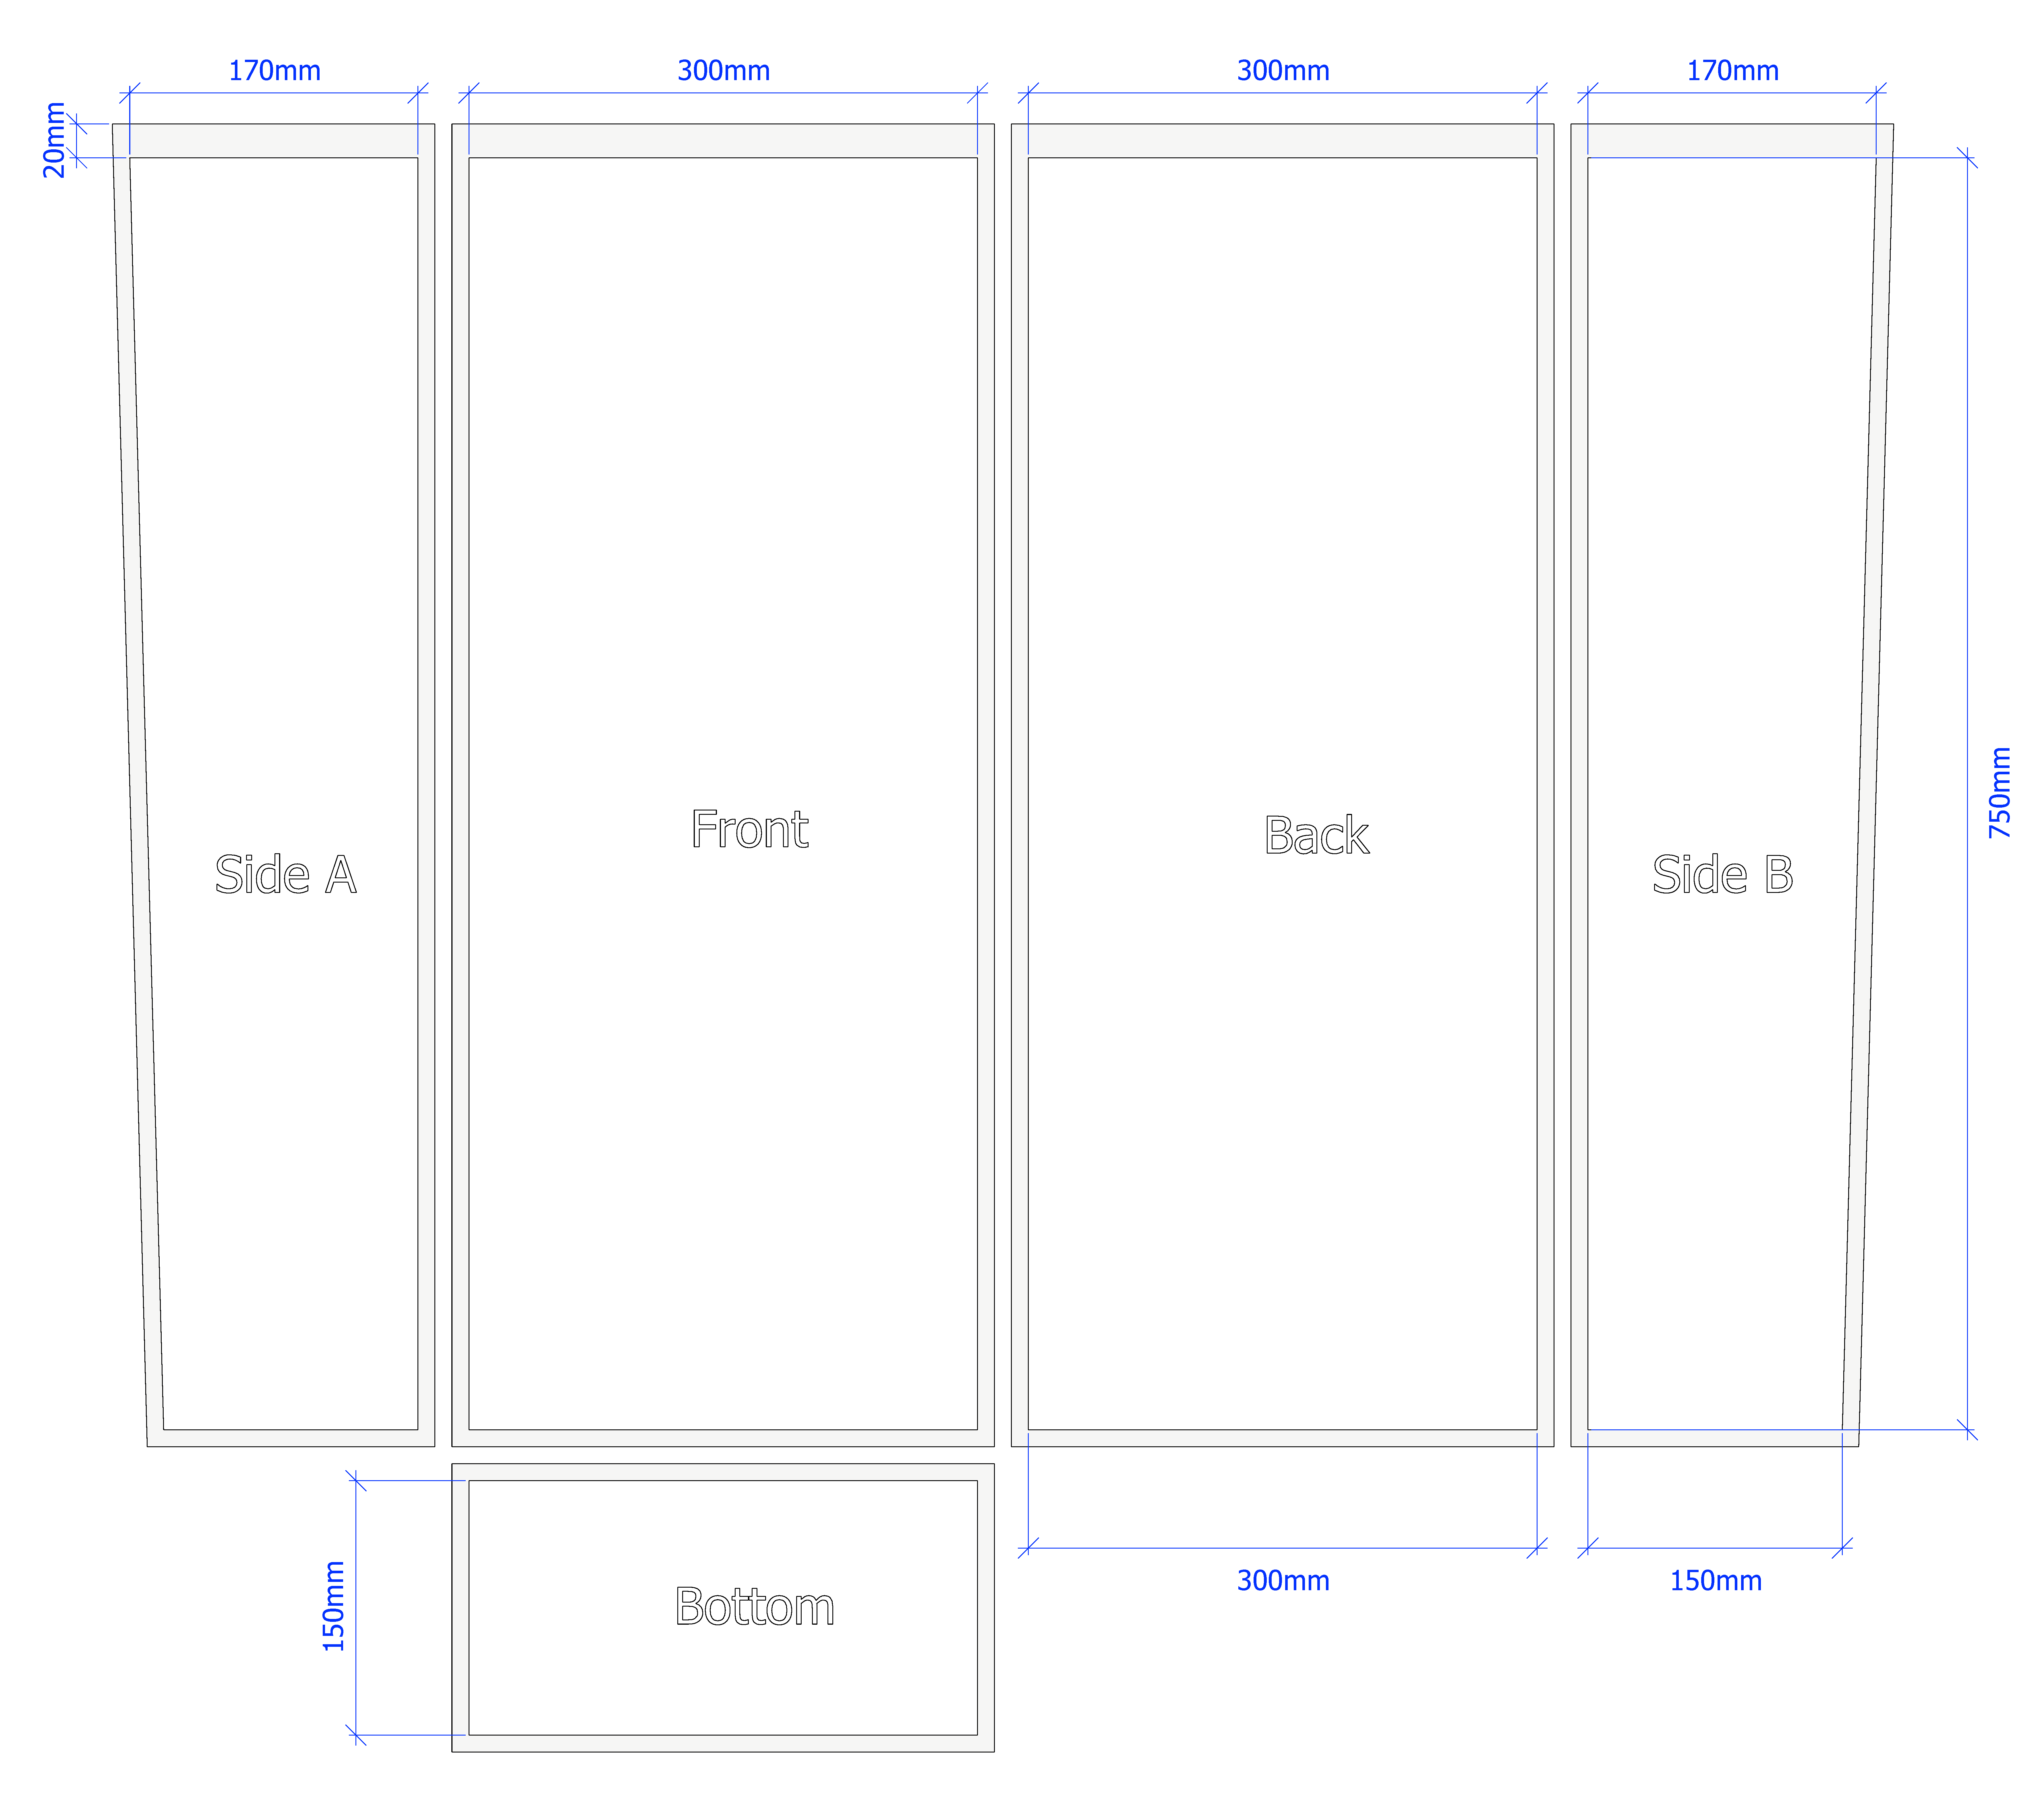
\includegraphics[width=\textwidth]{media/sketches/pack-rough-cut.pdf}
  \caption{Rough backpack dimensions including seam allowance of 10mm}
  \label{img:pack-rough-cut-2D}
\end{figure}

In the illustration \ref{img:pack-rough-cut-2D}, the golden ratio is not obvious, but it is there. If we look at the front panel, the golden ratio is only there in the assembled pack, and definitely not visible in the fabric cut ($\frac{750}{300} \gg 1.6$), but if you account for the ~20cm used for the roll-top and including some compression, you're getting pretty close ($\frac{550}{300} = 1.8$). I actually do prefer a slimmer backpack, but one could definitely get closer to the $1.6$ in any design.

I have tried many different combinations and ratios, and I find the best looks comes from ratios following constraints. These also account to some extent to my torso length (as I am slim and tall).

\begin{equation}
  1.65 < \varphi_{front} < 1.9
\end{equation}

With that in mind, my second constraint is given by the overall pack width I am aiming for, and that depends on my shoulder width. There is a very simple reason for that: it's not actually about the shoulder width itself (that accounts more for the straps design) but it is more about the freedom of movement of my arms. Let's say I'm hiking with trekking poles, I do not want my backpack to to be wider than my rib cage, and for my arms and elbows to constantly hit and rub on the pack all the time and create discomfort.

\begin{note}
  Seam allowance is crucial to the construction of a backpack. After experimenting a lot, I realised I tend to sew seams 10mm to 15mm from the side of the fabric. With that in mind, if I leave more than 15mm of fabric for the seem allowance - say 30mm - I would make a mess of my well thought pack dimensions because every seam would add overall 30mm extra fabric for each bond. That will end up in a much bigger pack than originally designed, and you definitely want to avoid that. I have ended up with a couple of backpacks that just look weird because of messed up dimensions. It's also the perfect allowance for binding the seams at a later stage with 20mm grosgrain ribbon.
\end{note}

\subsection{The front panel: aesthetics \& usability}

\begin{figure}[H]
  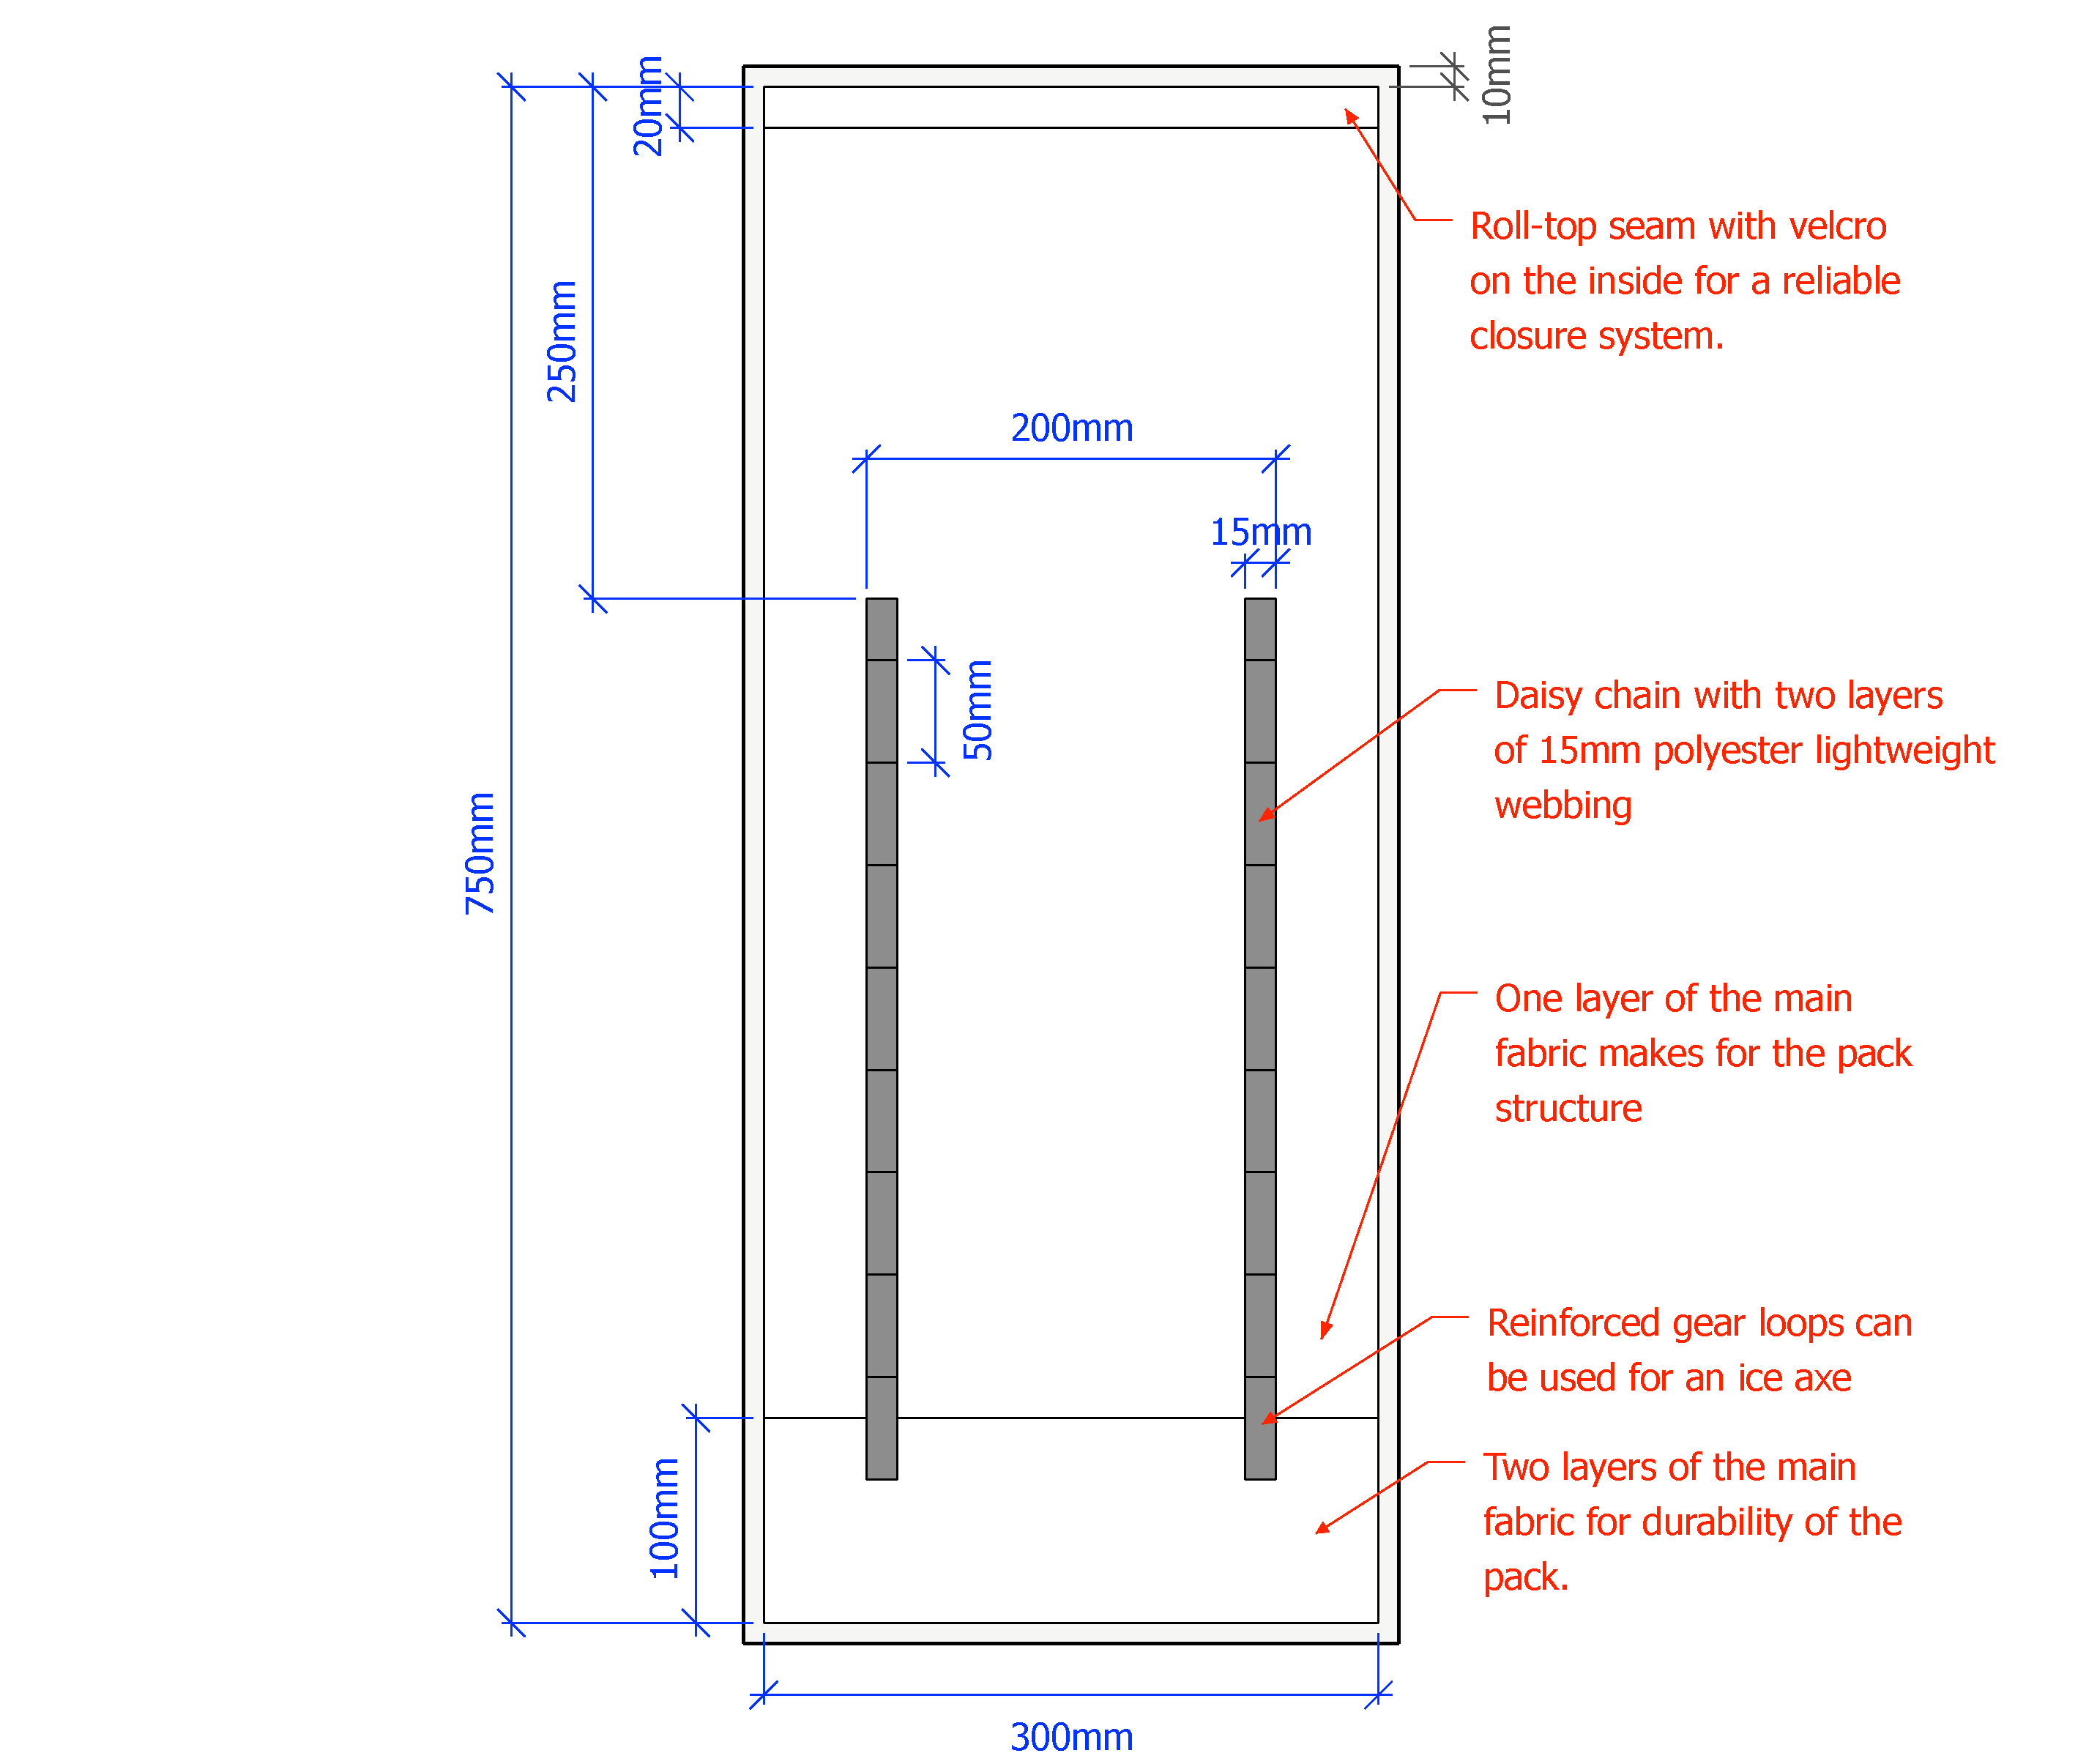
\includegraphics[width=\textwidth]{media/sketches/pack-front.pdf}
  \caption{Concept of the front panel designed for usbaility}
  \label{img:pack-front-2D}
\end{figure}

\subsection{The side panels: flexibility}
\subsection{The bottom panel: robustness}
\subsection{The back panel: comfort}
\subsection{The shoulder straps: lightweight}
\subsection{The hip belt: padding}
